%! Author = felix
%! Date = 17/03/2024

\renewcommand{\kapitelautor}{Autor: Felix Zwickelstorfer}
\subsection{Parser}\label{subsec:parser}
\renewcommand{\kapitelautor}{Autor: Felix Zwickelstorfer}

Der Parser nimmt einen Text in "raw" und zusätzlich eine Liste an Objekten, die beschreiben, wie dieser Text am Ende aussehen soll, beziehungsweise welche Besonderheiten vorkommen.
Dabei wird aus jedem vollständigen Wort (von einem Leerzeichen oder einem Zeilenumbruch getrennt) ein eigenes Element, was es erlaubt, den Text auf verschiedene Weisen hervorzuheben.
Weiters ist dadurch möglich, dass diese Elemente einen dynamischen Zeilenumbruch haben, falls sich der Text verändert.
Weiterhin gibt es die Möglichkeit, diverse Icons in den Text einzubinden.
Zusätzlich kann man den Text auf andere Weisen hervorheben als nur durch Schriftart und Größe, \zB durch das Bewegen des Textes.
Diese Funktionen kann man beispielsweise am Hovertext von der Deputies Bullet erkennen:
\begin{figure}[H]
    \centering
    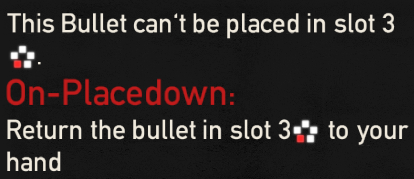
\includegraphics[width=0.7\textwidth]{hovertext_bulletbullet.png}
    \caption{Screenshot des Hovertexts der Deputies Bullet}
\end{figure}